\section*{(16\textordfeminine\ aula) --- Oscilador Harmônico (Cap. 7)}

\subsection*{A Hamiltoniana Clássica do Oscilador Harmônico}

A Hamiltoniana clássica de uma massa $m$, que se move em 1D sob a ação de uma força do tipo $F = -kx$, onde $x$ é a posição da partícula, é

\begin{equation}
    H(x,p) = \frac{p^2}{2m} + \frac{1}{2}kx^2
\label{eq:aula16_H_xp_k}
\end{equation}

Ou, usando $\omega = \sqrt{\dfrac{k}{m}}$,

\begin{equation}
    H(x,p) = \frac{p^2}{2m} + \frac{1}{2}m\omega^2 x^2 .
\label{eq:aula16_H_xp_omega}
\end{equation}

Essa Hamiltoniana aparece em inúmeras situações na Física pois ela é a forma \textbf{APROXIMADA} da Hamiltoniana de uma partícula que se move nas proximidades de um mínimo de um potencial $V(x)$ genérico.

\begin{center}
\begin{tikzpicture}[scale=1.1]
    \draw[->] (-0.3,0) -- (4.5,0) node[right] {$x$};
    \draw[->] (0,-0.3) -- (0,2.5) node[above] {$V(x)$};
    \draw[thick] (0,2.2) .. controls (1.0,-0.2) and (1.3,-0.2) .. (2.0,0.4)
                 .. controls (2.8,1.1) and (3.5,1.6) .. (4.2,2.3);
    \draw[dotted] (2.0,0) -- (2.0,0.4);
    \node[below] at (2.0,0) {$x_0$};
\end{tikzpicture}
\end{center}

\begin{equation}
    H(x,p) = \frac{p^2}{2m} + V(x), \quad \text{para movimentos próximos a } x_0
\label{eq:aula16_H_proximo_x0}
\end{equation}
\begin{equation}
    \simeq \frac{p^2}{2m} + V(x_0) + \overbrace{V'(x_0)}^{0}(x-x_0) + \frac{1}{2}V''(x_0)(x-x_0)^2 + \cdots
\label{eq:aula16_V_expansao}
\end{equation}

Eliminando a constante $V(x_0)$ temos uma Hamiltoniana de oscilador harmônico com ``constante de mola'' $k = V''(x_0)$ (derivada segunda do potencial no mínimo).

Se mudamos a origem do eixo $x$ para $x_0$ temos exatamente

\begin{equation}
    H(x,p) = \frac{p^2}{2m} + \frac{1}{2}kx^2 .
\label{eq:aula16_H_apos_translacao}
\end{equation}

\fbox{\parbox{0.92\textwidth}{
\textbf{Obs:} Não se deve perder de vista que essa forma da Hamiltoniana só é válida se $x$ permanecer próximo à origem (o ponto de equilíbrio). Para grandes deslocamentos, a força completa, com $V(x)$, deve ser usada.
}}

\subsection*{Modos Normais}

Quando temos um sistema com várias partículas em mais de 1 dimensão, encontramos situações próximas do equilíbrio descritas por Lagrangianas e Hamiltonianas na forma

\begin{equation}
    \mathcal{L}(\vec{q}, \dot{\vec{q}}) = \sum_{i=1}^{N}\sum_{j=1}^{N} \frac{1}{2}M_{ij}\dot{q}_i\dot{q}_j - \frac{1}{2}V_{ij}q_i q_j
\label{eq:aula16_lagrangiana_modos}
\end{equation}
\begin{equation}
    H(\vec{p}, \vec{q}) = \sum_{i=1}^{N}\sum_{j=1}^{N} \frac{1}{2}(M^{-1})_{ij}p_i p_j + \frac{1}{2}V_{ij}q_i q_j
\label{eq:aula16_hamiltoniana_modos}
\end{equation}
onde $M_{ij}$ e $V_{ij}$ são matrizes simétricas, e $q_i$ é a coordenada (não necessariamente cartesiana) correspondente ao deslocamento do ponto de equilíbrio.

Mudando as coordenadas: $\vec{q} = (q_1, q_2, \dots, q_N)$,

\begin{equation}
    \vec{q}(t) = \sum_{k=1}^{N} c_k(t)\,\vec{v}_k
\label{eq:aula16_mudanca_coordenadas}
\end{equation}
onde os $N$ vetores $\vec{v}_k$ são autovetores de

\begin{equation}
    \omega_k^2 \, M \, \vec{v}_k = V\, \vec{v}_k
\label{eq:aula16_autovetores}
\end{equation}
com ``ortonormalização''

\begin{equation}
    \vec{v}_k \cdot M \cdot \vec{v}_\ell = \delta_{k\ell} \qquad \text{e} \qquad \vec{v}_k \cdot V \cdot \vec{v}_\ell = \omega_k^2\,\delta_{k\ell}.
\label{eq:aula16_ortonormalizacao}
\end{equation}

A Lagrangiana para as novas coordenadas $c_k(t)$ é

\begin{equation}
    \mathcal{L}(\vec{c}, \dot{\vec{c}}) = \sum_{k=1}^{N} \left( \frac{1}{2}\dot{c}_k^2 - \frac{1}{2}\omega_k^2 c_k^2 \right)
\label{eq:aula16_lagrangiana_ck}
\end{equation}
igual a $N$ osciladores harmônicos 1D \underline{INDEPENDENTES}.

Isso justifica o interesse em conhecer, clássica e quanticamente, a solução do problema associado a

\begin{equation}
    H(x,p) = \frac{p^2}{2m} + \frac{1}{2}m\omega^2 x^2 .
\label{eq:aula16_H_problema_basico}
\end{equation}

\subsection*{Mecânica Clássica}

As equações de Hamilton para $x(t)$ e $p(t)$ são

\begin{equation}
    \dot{p} = -m\omega^2 x \qquad \text{e} \qquad \dot{x} = \frac{p}{m}.
\label{eq:aula16_eqs_hamilton_oh}
\end{equation}

Eliminando $p(t)$ obtemos a equação de Newton

\begin{equation}
    \ddot{x} = -\omega^2 x
\label{eq:aula16_newton}
\end{equation}
com solução

\begin{equation}
    x(t) = A\cos\omega t + B \sin\omega t,
\label{eq:aula16_solucao_classica}
\end{equation}
onde $A, B$ são determinados pelas condições iniciais $x(0)$ e $\dot{x}(0)$.

A Hamiltoniana é conservada (porque?) e é igual à energia cinética mais a energia potencial. Usando $p(t) = m\dot{x} = -m\omega A \sin\omega t + m\omega B\cos\omega t$ em

\begin{align}
    H &= \frac{p^2}{2m} + \frac{1}{2}m\omega^2 x^2 \notag \\
    &= \frac{1}{2m}\left(-m\omega A\sin\omega t + m\omega B \cos\omega t\right)^2 + \frac{1}{2}m\omega^2\left(A\cos\omega t + B \sin\omega t\right)^2 \notag \\
    &= \frac{1}{2}m\omega^2 (A^2 + B^2)
\label{eq:aula16_H_classica_AB}
\end{align}

A energia total pode ter qualquer valor $E \geq 0$.

\subsection*{Mecânica Quântica}

Como fizemos com todos os problemas até aqui, vamos começar procurando os autoestados e autovalores do operador

\begin{equation}
    \hat{H} = \frac{\hat{P}^2}{2m} + \frac{1}{2}m\omega^2 \hat{X}^2 .
\label{eq:aula16_H_operador}
\end{equation}

Da forma do potencial

\begin{center}
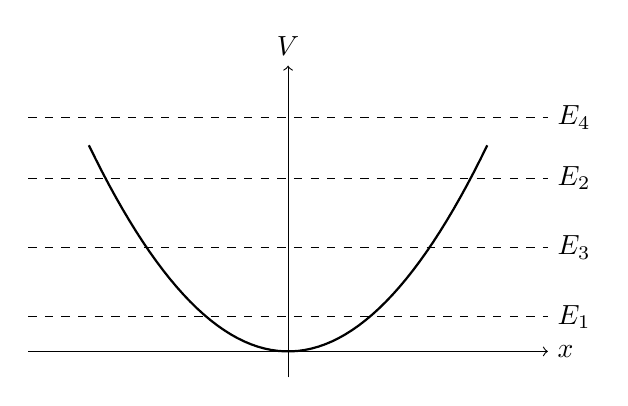
\begin{tikzpicture}[scale=1.1]
    \draw[->] (-3,0) -- (3,0) node[right] {$x$};
    \draw[->] (0,-0.3) -- (0,3.3) node[above] {$V$};
    \draw[thick] plot[domain=-2.3:2.3,samples=60] (\x, {0.45*\x*\x});
    \draw[dashed] (-3,0.4) -- (3,0.4) node[right] {$E_1$};
    \draw[dashed] (-3,1.2) -- (3,1.2) node[right] {$E_3$};
    \draw[dashed] (-3,2.0) -- (3,2.0) node[right] {$E_2$};
    \draw[dashed] (-3,2.7) -- (3,2.7) node[right] {$E_4$};
\end{tikzpicture}
\end{center}

vemos que os autovalores são \textbf{DISCRETOS}, \textbf{NÃO-DEGENERADOS} e \textbf{POSITIVOS} (você sabe porquê?).

Até agora só vimos potenciais constantes aos pedaços (i.e. descontínuos)

\begin{center}
\begin{tikzpicture}[scale=1.0]
    \draw[->] (-0.3,0) -- (3.5,0) node[right] {$x$};
    \draw[->] (0,-0.3) -- (0,2) node[above] {$V(x)$};
    \draw[thick] (0,0) -- (1,0) -- (1,1.2) node[above] {$V_0$} -- (2,1.2) -- (2,0) -- (3.5,0);
\end{tikzpicture}
\hspace{1.5cm}
\begin{tikzpicture}[scale=1.0]
    \draw[->] (-0.3,0) -- (3.5,0) node[right] {$x$};
    \draw[->] (0,-0.3) -- (0,2) node[above] {$V(x)$};
    \draw[thick] (0,0) -- (1.2,0) -- (1.2,1.2) node[above] {$V_0$} -- (1.8,1.2) -- (1.8,0) -- (3.5,0);
    \node[right] at (3.5,0) {etc.};
\end{tikzpicture}
\end{center}

O potencial harmônico fornece uma equação de autovalor na forma

\begin{equation}
    \hat{H}\ket{E} = E\ket{E}
\label{eq:aula16_eq_autovalor_ket}
\end{equation}
\begin{equation}
    \Longrightarrow \quad -\frac{\hbar^2}{2m}\frac{d^2\psi_E}{dx^2} + \frac{1}{2}m\omega^2 x^2 \psi_E(x) = E\,\psi_E(x)
\label{eq:aula16_eq_schrodinger_oh}
\end{equation}
válida em todo o eixo-$x$.

Essa equação pode ser resolvida para qualquer valor de $E$, mas apenas \textbf{CERTOS VALORES DE $E$} têm como solução funções $\psi_E(x)$ que $\to 0$ quando $x \to \pm\infty$.

Vamos encontrar os autovalores $E$ e as autofunções $\psi_E(x)$ usando uma técnica de série de potências que será útil em outros casos (por exemplo no caso do potencial coulombiano).

\subsection*{1 --- Torne a EDO adimensional}

Fazemos $x = by$, onde $y$ é a variável adimensional e $b$ é uma unidade de comprimento.

\begin{equation}
    \psi_E(x) = \psi_E(by)
\label{eq:aula16_mudanca_variavel}
\end{equation}
\begin{equation}
    \frac{d\psi_E}{dx} = \frac{d\psi_E}{dy}\frac{dy}{dx} = \frac{d\psi_E}{dy}\frac{1}{b}
\label{eq:aula16_derivada_cadeia}
\end{equation}

Substituindo na equação de Schrödinger,

\begin{equation}
    -\frac{\hbar^2}{2mb^2}\frac{d^2\psi_E}{dy^2} + \frac{1}{2}m\omega^2 b^2 y^2 \psi_E = E\,\psi_E
\label{eq:aula16_eq_em_y}
\end{equation}
\begin{equation}
    \psi_E'' + \left( \underbrace{\frac{2mEb^2}{\hbar^2}}_{\text{sem dimensão}} - \underbrace{\frac{m^2\omega^2 b^4}{\hbar^2}y^2}_{\text{sem dimensão}} \right)\psi_E = 0
\label{eq:aula16_eq_adim_intermediaria}
\end{equation}

Escolhemos $b = \sqrt{\dfrac{\hbar}{m\omega}}$ para tornar o segundo termo igual a $1$, e definimos a energia adimensional

\begin{equation}
    \varepsilon = \frac{mb^2 E}{\hbar^2} = \frac{E}{\hbar\omega}.
\label{eq:aula16_energia_adimensional}
\end{equation}

Assim temos a EDO adimensional

\begin{equation}
    \boxed{\psi_E'' + (2\varepsilon - y^2)\psi_E = 0}
\label{eq:aula16_edo_adimensional}
\end{equation}

Queremos encontrar os valores de $\varepsilon$ que têm como solução $\psi_E(y)$ tal que $\psi_E \to 0$ quando $y \to \pm\infty$.

\subsection*{Análise Assintótica}

Como essa EDO não é conhecida, analisamos a forma de sua solução (para um $\varepsilon$ genérico) em $y \to 0$ e $|y| \to \infty$.

\begin{align}
    y \to 0: \quad \psi_E'' + 2\varepsilon\,\psi_E = 0 \;&\Longrightarrow\; \psi_E(y) = A\cos\left(\sqrt{2\varepsilon}\,y\right) + B\sin\left(\sqrt{2\varepsilon}\,y\right) \notag \\
    &\simeq A + B\sqrt{2\varepsilon}\,y + O(y^2)
\label{eq:aula16_assintotica_y0}
\end{align}

\begin{align}
    |y| \to \infty: \quad \psi_E'' - y^2 \psi_E &= 0 \notag \\
    \psi_E(y) = y^m e^{\pm y^2/2} \quad &\text{satisfaz essa equação \textbf{NESSE LIMITE}} \notag \\
    \psi_E''(y) = y^{m+2}e^{\pm y^2/2}\left( 1 \pm \frac{2m+1}{y} + \frac{m(m-1)}{y^2} \right) &\simeq y^2 \psi_E(y)
\label{eq:aula16_assintotica_infinito}
\end{align}

Essas análises mostram que, para um $\varepsilon$ \textbf{GENÉRICO},

\begin{equation}
    \psi_E \to
    \begin{cases}
        A + By & y \to 0 \quad \text{(regular na origem)} \\
        y^m e^{\pm y^2/2} & |y| \to \infty
    \end{cases}
\label{eq:aula16_comportamento_geral}
\end{equation}

Quando $\varepsilon$ \textbf{NÃO} corresponde a um autovalor, as 2 soluções independentes divergem no infinito como $y^m e^{y^2/2}$ e $y^n e^{y^2/2}$. Quando $\varepsilon$ é um dos autovalores, uma das soluções vai como $y^m e^{-y^2/2}$ (e a outra continua divergindo como $y^n e^{y^2/2}$).

\subsection*{Série de Potências}

Usamos $\psi_E(y) = u(y)\,e^{-y^2/2}$ na EDO.

\begin{equation}
    \psi_E'' = \left[u'' - 2yu' + (y^2-1)u\right]e^{-y^2/2}
\label{eq:aula16_psi_segunda_derivada}
\end{equation}
e obtemos a seguinte EDO para $u(y)$:

\begin{equation}
    \boxed{u'' - 2yu' + (2\varepsilon - 1)u = 0}
\label{eq:aula16_edo_u}
\end{equation}

Essa EDO, diferentemente da $\psi_E'' + (2\varepsilon - y^2)\psi_E = 0$, se presta à solução por série de potências

\begin{equation}
    u(y) = \sum_{n=0}^{\infty} c_n y^n \qquad \text{(regular na origem!)}
\label{eq:aula16_serie_potencias}
\end{equation}

\begin{equation}
    \sum_{n=0}^{\infty} n(n-1)c_n y^{n-2} - 2n\,c_n y^n + (2\varepsilon - 1)c_n y^n = 0
\label{eq:aula16_serie_substituida}
\end{equation}

reescrevemos a 1\textsuperscript{a} série como

\begin{align}
    \sum_{n=0}^{\infty} n(n-1)c_n y^{n-2} &= \sum_{n=2}^{\infty} n(n-1)c_n y^{n-2} \notag \\
    &= \sum_{m=0}^{\infty} (m+2)(m+1)c_{m+2}\, y^m
\label{eq:aula16_reescrita_serie}
\end{align}

\begin{equation}
    \sum_{n=0}^{\infty} \left[ (n+2)(n+1)c_{n+2} - (2n+1-2\varepsilon)c_n \right] y^n = 0
\label{eq:aula16_serie_colchetes}
\end{equation}

O termo entre colchetes deve ser nulo, e obtemos uma relação entre $c_n$ e $c_{n+2}$ $\Rightarrow$ por isso a EDO se presta à solução por séries!

Tratamos $c_0$ e $c_1$ como as 2 constantes arbitrárias e encontramos

\begin{align}
    \psi(y) = \; &c_0\left[ 1 + \frac{(1-2\varepsilon)}{2}y^2 + \frac{(1-2\varepsilon)(5-2\varepsilon)}{2\cdot 12}y^4 + \cdots \right]e^{-y^2/2} \notag \\
    + \; &c_1\left[ y + \frac{(3-2\varepsilon)}{6}y^3 + \frac{(3-2\varepsilon)(7-2\varepsilon)}{6\cdot 24}y^5 + \cdots \right]e^{-y^2/2}
\label{eq:aula16_solucao_serie}
\end{align}
onde usei

\begin{equation}
    \boxed{c_{n+2} = \frac{2n+1-2\varepsilon}{(n+2)(n+1)}c_n}
\label{eq:aula16_relacao_recorrencia}
\end{equation}
para obter $\{c_2, c_4, c_6, \dots\}$ em termos de $c_0$ e $\{c_3, c_5, c_7, \dots\}$ em termos de $c_1$.

Essa é a solução geral de $\psi'' + (2\varepsilon - y^2)\psi = 0$ para um $\varepsilon$ genérico.

Veja que se $2\varepsilon = \{1,3,5,\dots\}$ um dos dois colchetes se torna um polinômio \textbf{FINITO} e obtemos uma solução que pertence à classe de funções da MQ (e que multiplicado é $y^n e^{-y^2/2}$).

Caso $2\varepsilon \neq \{1,3,5,\dots\}$, \textbf{AMBAS} as soluções divergem no infinito como $y^m e^{y^2/2}$ (isso pode não ser óbvio mas é demonstrável).

\subsection*{Autoenergias e Autofunções}

\begin{equation}
    \text{AUTOENERGIAS:} \quad 2\varepsilon = 2n+1 \qquad (n=0,1,2,\dots)
\label{eq:aula16_autoenergias_condicao}
\end{equation}

\begin{equation}
    \frac{2E}{\hbar\omega} = 2n+1 \;\Longrightarrow\; \boxed{E = \left(n+\frac{1}{2}\right)\hbar\omega}
\label{eq:aula16_autoenergias_final}
\end{equation}

AUTOFUNÇÕES (não normalizadas):

\begin{align}
    n=0 \;\; (2\varepsilon=1): \quad &\psi_0(y) = e^{-y^2/2} \notag \\
    n=1 \;\; (2\varepsilon=3): \quad &\psi_1(y) = y\,e^{-y^2/2} \notag \\
    n=2 \;\; (2\varepsilon=5): \quad &\psi_2(y) = (1-2y^2)\,e^{-y^2/2} \notag \\
    n=3 \;\; (2\varepsilon=7): \quad &\psi_3(y) = \left(y - \frac{2}{3}y^3\right)e^{-y^2/2}, \quad \text{etc.}
\label{eq:aula16_autofuncoes_lista}
\end{align}

\subsection*{Polinômios de Hermite}

Esses polinômios multiplicando $e^{-y^2/2}$ são os \textbf{POLINÔMIOS DE HERMITE}. Sua definição correta é

\begin{align}
    H_0(y) &= 1 \notag \\
    H_1(y) &= 2y \notag \\
    H_2(y) &= -2(1-2y^2) \notag \\
    H_3(y) &= -12\left(y - \frac{2}{3}y^3\right) \notag \\
    H_4(y) &= 12\left(1 - 4y^2 + \frac{4}{3}y^4\right), \quad \text{etc.}
\label{eq:aula16_hermite_lista}
\end{align}

Basta lembrar $H_0$ e $H_1$ pois a \textbf{FÓRMULA DE RECORRÊNCIA} determina os demais

\begin{equation}
    \boxed{H_{n+1} = 2y H_n - 2n H_{n-1}}
\label{eq:aula16_hermite_recorrencia}
\end{equation}

Temos também a relação de ortogonalidade:

\begin{equation}
    \int_{-\infty}^{\infty} H_n(y) H_m(y)\, e^{-y^2}\, dy = \delta_{mn}\left(\sqrt{\pi}\,2^n n!\right),
\label{eq:aula16_hermite_ortogonalidade}
\end{equation}

que faz com que as autofunções \textbf{NORMALIZADAS} do oscilador harmônico sejam

\begin{equation}
    \boxed{\psi_n(x) = \frac{1}{\sqrt{b}}\left(\frac{1}{\sqrt{\pi}\,2^n n!}\right)^{1/2} H_n(x/b)\, e^{-x^2/2b^2}}
\label{eq:aula16_autofuncoes_normalizadas}
\end{equation}
onde $b = \sqrt{\dfrac{\hbar}{m\omega}}$.

\subsection*{Estado Fundamental e Primeiro Estado Excitado}

\begin{center}
\begin{minipage}{0.45\textwidth}
\centering
$E_0 = \dfrac{\hbar\omega}{2}$

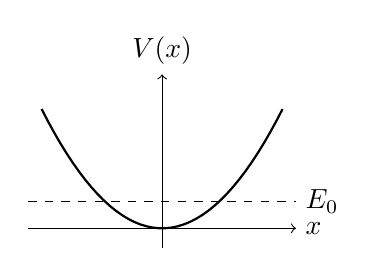
\begin{tikzpicture}[scale=0.85]
    \draw[->] (-2,0) -- (2,0) node[right] {$x$};
    \draw[->] (0,-0.3) -- (0,2.3) node[above] {$V(x)$};
    \draw[thick] plot[domain=-1.8:1.8,samples=40] (\x,{0.55*\x*\x});
    \draw[dashed] (-2,0.4) -- (2,0.4) node[right] {$E_0$};
\end{tikzpicture}

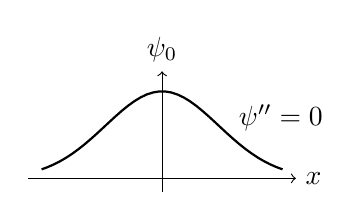
\begin{tikzpicture}[scale=0.85]
    \draw[->] (-2,0) -- (2,0) node[right] {$x$};
    \draw[->] (0,-0.2) -- (0,1.6) node[above] {$\psi_0$};
    \draw[thick] plot[domain=-1.8:1.8,samples=40] (\x,{1.3*exp(-0.7*\x*\x)});
    \node[right] at (1.0,0.9) {$\psi''=0$};
\end{tikzpicture}
\end{minipage}
\hfill
\begin{minipage}{0.45\textwidth}
\centering
$E_1 = \dfrac{3\hbar\omega}{2}$

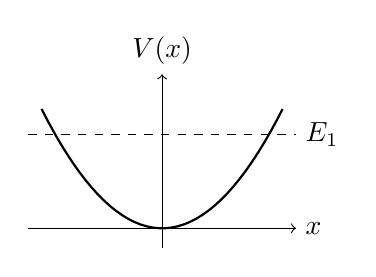
\begin{tikzpicture}[scale=0.85]
    \draw[->] (-2,0) -- (2,0) node[right] {$x$};
    \draw[->] (0,-0.3) -- (0,2.3) node[above] {$V(x)$};
    \draw[thick] plot[domain=-1.8:1.8,samples=40] (\x,{0.55*\x*\x});
    \draw[dashed] (-2,1.4) -- (2,1.4) node[right] {$E_1$};
\end{tikzpicture}

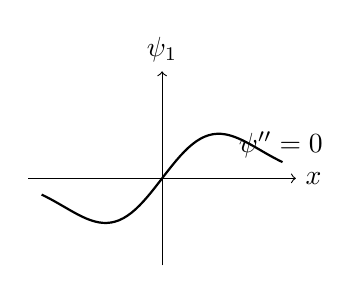
\begin{tikzpicture}[scale=0.85]
    \draw[->] (-2,0) -- (2,0) node[right] {$x$};
    \draw[->] (0,-1.3) -- (0,1.6) node[above] {$\psi_1$};
    \draw[thick] plot[domain=-1.8:1.8,samples=60] (\x,{1.3*\x*exp(-0.7*\x*\x)});
    \node[right] at (1.0,0.5) {$\psi''=0$};
\end{tikzpicture}
\end{minipage}
\end{center}

$\to$ Note o comportamento oscilatório na região classicamente permitida e o decaimento na região proibida.

$\to$ Note que para $n$ par a função é par, $\psi_n(x) = \psi_n(-x)$, enquanto para $n$ ímpar a função é ímpar, $\psi_n(x) = -\psi_n(-x)$.

Isso ajuda a calcular alguns integrais como

\begin{equation}
    \bra{4}\hat{X}\ket{6} = \int_{-\infty}^{\infty} \underbrace{\psi_4(x)}_{\text{par}} \, x \, \underbrace{\psi_6(x)}_{\text{par}}\, dx = 0
\label{eq:aula16_exemplo_integral_paridade}
\end{equation}

Existe uma outra fórmula de recorrência útil entre os polinômios de Hermite

\begin{equation}
    \boxed{H_n' = 2n\,H_{n-1}}
\label{eq:aula16_hermite_derivada}
\end{equation}

Use isso em cálculos envolvendo o operador $\hat{P}$.

Por exemplo:

\begin{align}
    \frac{d}{dx}\psi_5(x/b) &= \frac{1}{b}\frac{d}{dy}\left[ A_5 H_5(y) e^{-y^2/2} \right] \qquad (A_5: \text{const. de normalização}) \notag \\
    &= \frac{A_5}{b}\left[ 10\,H_4(y) - y\,H_5(y) \right] e^{-y^2/2}
\label{eq:aula16_exemplo_derivada_hermite}
\end{align}

Portanto a energia de um oscilador harmônico é \textbf{QUANTIZADA} em múltiplos de $\hbar\omega$. Além disso a menor energia possível de ser encontrada em uma medida é $\dfrac{\hbar\omega}{2}$, a energia do \textbf{ESTADO FUNDAMENTAL}.

\subsection*{Comparação com a Caixa Infinita}

A situação no potencial harmônico é semelhante à encontrada na caixa infinita.

\begin{center}
\begin{minipage}{0.45\textwidth}
\centering
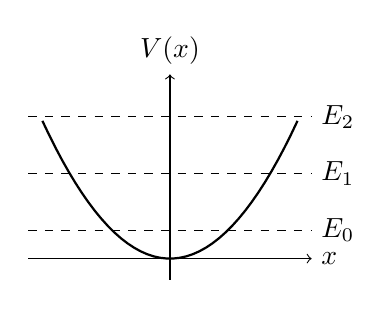
\begin{tikzpicture}[scale=0.9]
    \draw[->] (-2,0) -- (2,0) node[right] {$x$};
    \draw[->] (0,-0.3) -- (0,2.6) node[above] {$V(x)$};
    \draw[thick] plot[domain=-1.8:1.8,samples=40] (\x,{0.6*\x*\x});
    \draw[dashed] (-2,0.4) -- (2,0.4) node[right] {$E_0$};
    \draw[dashed] (-2,1.2) -- (2,1.2) node[right] {$E_1$};
    \draw[dashed] (-2,2.0) -- (2,2.0) node[right] {$E_2$};
    \node[right,align=left] at (2.3,1.2) {};
\end{tikzpicture}

$\boxed{E_n = \left(n+\tfrac{1}{2}\right)\hbar\omega} \quad (n=0,1,2,\dots)$

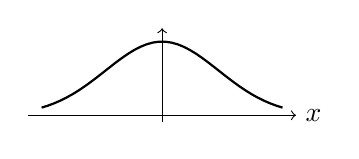
\begin{tikzpicture}[scale=0.85]
    \draw[->] (-2,0) -- (2,0) node[right] {$x$};
    \draw[->] (0,-0.1) -- (0,1.3);
    \draw[thick] plot[domain=-1.8:1.8,samples=40] (\x,{1.1*exp(-0.7*\x*\x)});
\end{tikzpicture}
\\ estado fundamental
\end{minipage}
\hfill
\begin{minipage}{0.45\textwidth}
\centering
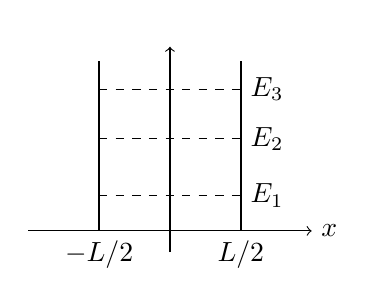
\begin{tikzpicture}[scale=0.9]
    \draw[->] (-2,0) -- (2,0) node[right] {$x$};
    \draw[->] (0,-0.3) -- (0,2.6) node[above] {};
    \draw[thick] (-1,0) -- (-1,2.4);
    \draw[thick] (1,0) -- (1,2.4);
    \draw[dashed] (-1,0.5) -- (1,0.5) node[right] {$E_1$};
    \draw[dashed] (-1,1.3) -- (1,1.3) node[right] {$E_2$};
    \draw[dashed] (-1,2.0) -- (1,2.0) node[right] {$E_3$};
    \node[below] at (-1,0) {$-L/2$};
    \node[below] at (1,0) {$L/2$};
\end{tikzpicture}

$\boxed{E_n = \dfrac{n^2\pi^2\hbar^2}{2mL^2}} \quad (n=1,2,3,\dots)$

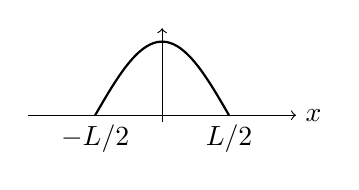
\begin{tikzpicture}[scale=0.85]
    \draw[->] (-2,0) -- (2,0) node[right] {$x$};
    \draw[->] (0,-0.1) -- (0,1.3);
    \draw[thick] plot[domain=-1:1,samples=40] (\x,{1.1*cos(90*\x)});
    \node[below] at (-1,0) {$-L/2$};
    \node[below] at (1,0) {$L/2$};
\end{tikzpicture}
\end{minipage}
\end{center}

apenas na caixa os níveis de energia não são uniformemente espaçados.

\subsection*{Combinação Linear de Autoestados}

Os autoestados do operador $\hat{H}$ são os estados de energia bem definida. Assim, por exemplo, no estado (normalizado)

\begin{equation}
    \ket{\Psi} = \frac{1}{\sqrt{6}}\ket{0} + \frac{2}{\sqrt{6}}\ket{2} + \frac{1}{\sqrt{6}}\ket{7}
\label{eq:aula16_estado_combinacao}
\end{equation}

em uma medida de energia, só podemos encontrar

\begin{center}
\begin{tabular}{ll}
    $\dfrac{\hbar\omega}{2}$, & com probabilidade $1/6$ \\[2mm]
    $\dfrac{5\hbar\omega}{2}$, & com probabilidade $4/6$ \\[2mm]
    $\dfrac{15\hbar\omega}{2}$, & com probabilidade $1/6$
\end{tabular}
\end{center}

\subsection*{Operador de Evolução e Propagador}

Esses autoestados permitem a construção do operador de evolução e do propagador desse Hamiltoniano.

\begin{equation}
    \hat{U}(t) = \sum_{n=0}^{\infty} e^{-iE_n t/\hbar}\ket{n}\bra{n} \qquad \left(E_n = \left(n+\tfrac{1}{2}\right)\hbar\omega\right)
\label{eq:aula16_operador_evolucao}
\end{equation}

\begin{equation}
    \bra{x}\hat{U}(t)\ket{x'} = \sum_{n=0}^{\infty} e^{-iE_n t/\hbar} A_n^2 H_n(x/b) H_n(x'/b)\, e^{-(x^2+x'^2)/2b^2}
\label{eq:aula16_propagador_serie}
\end{equation}

isso pode ser somado e é igual a (com $b = \sqrt{\hbar/m\omega}$)

\begin{equation}
    \boxed{U(x,x';t) = \left( \frac{1}{b^2 2\pi i \sin\omega t} \right)^{1/2} \exp\left[ \frac{i}{b^2}\frac{(x^2+x'^2)\cos\omega t - 2xx'}{2\sin\omega t} \right]}
\label{eq:aula16_propagador_fechado}
\end{equation}

Com o propagador podemos conhecer (a princípio) a evolução de qualquer estado inicial $\Psi(x,0)$

\begin{equation}
    \Psi(x,t) = \int_{-\infty}^{\infty} dx' \, U(x,x';t)\,\Psi(x',0)
\label{eq:aula16_evolucao_via_propagador}
\end{equation}

\subsection*{Limite Clássico}

\textbf{LIMITE CLÁSSICO} --- No caso do potencial quadrático, o teorema de Ehrenfest diz que os valores médios

\begin{equation}
    \langle x(t) \rangle = \bra{\Psi(t)} \hat{X} \ket{\Psi(t)} \qquad \text{e} \qquad \langle p(t) \rangle = \bra{\Psi(t)} \hat{P} \ket{\Psi(t)}
\label{eq:aula16_ehrenfest_valores_medios}
\end{equation}

de \textbf{QUALQUER} $\ket{\Psi(t)}$ que evolua com o $\hat{H}$ do oscilador harmônico obedecem às equações clássicas.

\begin{equation}
    \frac{d\langle x \rangle}{dt} = \frac{\langle p \rangle}{m} \qquad \text{(qualquer potencial tem essa propriedade)}
\label{eq:aula16_ehrenfest_dxdt}
\end{equation}

\begin{equation}
    \frac{d\langle p \rangle}{dt} = \underbrace{F(\langle x \rangle)}_{\text{força}} \qquad \text{(apenas os potenciais quadrático, linear e constante têm essa propriedade; em geral o lado direito é } \langle F(x) \rangle \text{)}
\label{eq:aula16_ehrenfest_dpdt}
\end{equation}

No caso de um ``pacote clássico'' gaussiano

\begin{equation}
    \Psi(x,0) = \left( \frac{1}{\pi\Delta^2} \right)^{1/4} e^{ip_0 x/\hbar}\, e^{-(x-x_0)^2/2\Delta^2}
\label{eq:aula16_pacote_gaussiano}
\end{equation}

veremos a evolução no tempo

\begin{center}
\begin{tikzpicture}[scale=1.0]
    \draw[->] (-3.5,0) -- (3.5,0) node[right] {$x$};
    \draw[thick] (-2.6,0) ellipse (0.25 and 0.5);
    \draw[->] (-2.3,0.8) -- (-1.7,0.8) node[above] {$p_0/m$};
    \node[below] at (-2.6,0) {$x_0$};
    \node[below] at (-3.2,0) {$-A$};
    \node[below] at (0,0) {$O$};
    \node[below] at (3.2,0) {$A$};
\end{tikzpicture}
\hfill
\begin{tikzpicture}[scale=1.0]
    \draw[->] (-3.5,0) -- (3.5,0) node[right] {$x$};
    \draw[thick] (1.6,0) ellipse (0.55 and 0.35);
    \node[above] at (0.3,0.6) {$\to \;\;\leftarrow$};
    \node[below] at (0,0) {$O$};
    \node[below] at (3.2,0) {$A$};
\end{tikzpicture}
\hfill
\begin{tikzpicture}[scale=1.0]
    \draw[->] (-3.5,0) -- (3.5,0) node[right] {$x$};
    \draw[thick] (2.6,0) ellipse (0.25 and 0.5);
    \draw[->] (2.3,0.8) -- (1.7,0.8) node[above] {$v_{\max}$};
    \node[below] at (0,0) {$O$};
\end{tikzpicture}
\end{center}

O valor médio $\langle x \rangle$ oscila exatamente como a partícula clássica e a força (o pacote se alarga e se estreita durante a oscilação).

\subsection*{Quantização Imperceptível para Massas/Sistemas Grandes}

Além disso, a quantização dos níveis de energia é \textbf{IMPERCEPTÍVEL} no caso de massas grandes.

Imagine uma massa pequena e uma grande sob a ação de um mesmo potencial $V(x) = \dfrac{1}{2}kx^2$

\begin{center}
\begin{minipage}{0.45\textwidth}
\centering
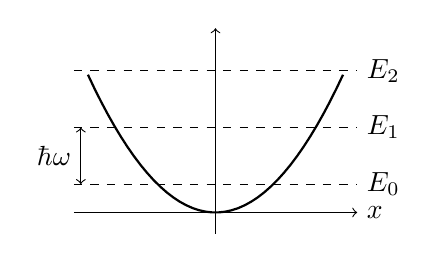
\begin{tikzpicture}[scale=0.9]
    \draw[->] (-2,0) -- (2,0) node[right] {$x$};
    \draw[->] (0,-0.3) -- (0,2.6);
    \draw[thick] plot[domain=-1.8:1.8,samples=40] (\x,{0.6*\x*\x});
    \draw[dashed] (-2,0.4) -- (2,0.4) node[right] {$E_0$};
    \draw[dashed] (-2,1.2) -- (2,1.2) node[right] {$E_1$};
    \draw[dashed] (-2,2.0) -- (2,2.0) node[right] {$E_2$};
    \draw[<->] (-1.9,0.4) -- (-1.9,1.2) node[midway,left] {$\hbar\omega$};
\end{tikzpicture}
\\ (m pequena)
\end{minipage}
\hfill
\begin{minipage}{0.45\textwidth}
\centering
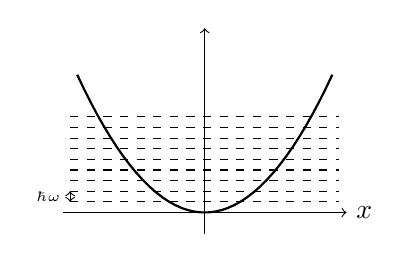
\begin{tikzpicture}[scale=0.9]
    \draw[->] (-2,0) -- (2,0) node[right] {$x$};
    \draw[->] (0,-0.3) -- (0,2.6);
    \draw[thick] plot[domain=-1.8:1.8,samples=40] (\x,{0.6*\x*\x});
    \foreach \y in {0.15,0.3,...,1.5} {
        \draw[dashed] (-1.9,\y) -- (1.9,\y);
    }
    \draw[<->] (-1.9,0.15) -- (-1.9,0.3) node[midway,left] {\tiny $\hbar\omega$};
\end{tikzpicture}
\\ (m grande)
\end{minipage}
\end{center}

Isso ocorre pois $\hbar\omega = \hbar\sqrt{\dfrac{k}{m}}$ é o espaçamento dos níveis.

O mesmo ocorre no poço infinito. Imagine uma massa grande e uma pequena confinadas em uma região de tamanho $L$.

\begin{center}
\begin{minipage}{0.45\textwidth}
\centering
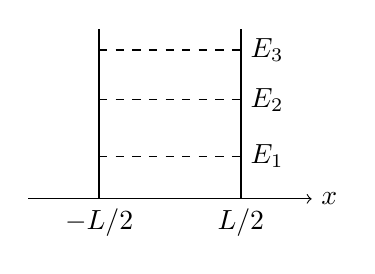
\begin{tikzpicture}[scale=0.9]
    \draw[->] (-2,0) -- (2,0) node[right] {$x$};
    \draw[thick] (-1,0) -- (-1,2.4);
    \draw[thick] (1,0) -- (1,2.4);
    \draw[dashed] (-1,0.6) -- (1,0.6) node[right] {$E_1$};
    \draw[dashed] (-1,1.4) -- (1,1.4) node[right] {$E_2$};
    \draw[dashed] (-1,2.1) -- (1,2.1) node[right] {$E_3$};
    \node[below] at (-1,0) {$-L/2$};
    \node[below] at (1,0) {$L/2$};
\end{tikzpicture}
\\ (m pequena)
\end{minipage}
\hfill
\begin{minipage}{0.45\textwidth}
\centering
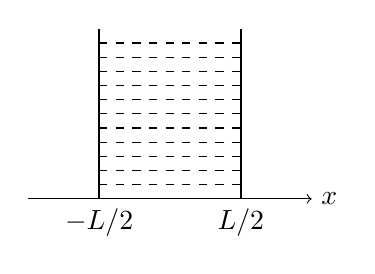
\begin{tikzpicture}[scale=0.9]
    \draw[->] (-2,0) -- (2,0) node[right] {$x$};
    \draw[thick] (-1,0) -- (-1,2.4);
    \draw[thick] (1,0) -- (1,2.4);
    \foreach \y in {0.2,0.4,...,2.2} {
        \draw[dashed] (-1,\y) -- (1,\y);
    }
    \node[below] at (-1,0) {$-L/2$};
    \node[below] at (1,0) {$L/2$};
\end{tikzpicture}
\\ (m grande)
\end{minipage}
\end{center}

Isso ocorre pois $E_n = \dfrac{n^2\pi^2\hbar^2}{2mL^2}$ é inversamente proporcional à massa.
